\subsection*{Fejlmeddelelse}
Til at vise fejlmeddelelser er der opstillet en fælles grænseflade, hvori teksten ændres alt efter, hvilken fejl, der forekommer. Designklassen ses af \autoref{fig:Designfejl}.

\begin{figure} [H]
\centering
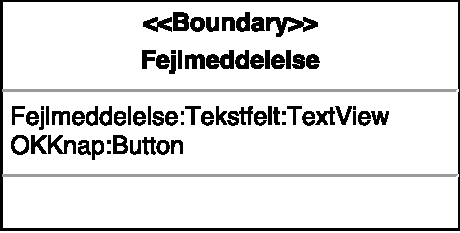
\includegraphics[width=0.9\textwidth]{figures/MVC/MVCfejl}
\caption{Designklasse for fejlmeddelelse.}
\label{fig:Designfejl}
\end{figure}

\noindent
Grænsefladen indeholder, foruden et tekstfelt, en OKKnap, der ved tryk henviser systemet til den forhenværende grænseflade. Fejlmeddelelsesgrænsefladen håndteres af den pågældende controller, hvori fejlen opstår. 